%********************************************************************************************
%								COMANDOS ÚTILES PARA LATEX EN ESTE TP							
%
%	\ : espacio simple
%	\\ : nueva línea
%	\par : va a la línea de abajo y deja sangría
%	\vspace{##tamaño en pt##} o \vspace{\baselineskip} en general:
%								 para dejar un espacio vertical
%	\textbf{text} :text en negrita
%	\textit{text} :text en itálica
%
% GRAFICOS CENTRADOS:
%	\begin{center}
%		\includegraphics[width=\textwidth]{./img/##ruta imagen (no hace falta extension)##}
%	\end{center}
%		--> se pueden agregar atributos como scale por si se hace muy grande
%
% TABLAS CENTRADAS:
%	\begin{center}
%	\begin{tabular}{|c|c|}
%	\hline
%	\ \textbf{Programa} & \textbf{Ticks} \\
%	\hline
%		ASM & 675127609 \\
%	\hline
%	\end{tabular}
%	\end{center}
%
% ALGORITMOS (EN VARIOS LENGUAJES):
% \begin{lstlisting}
%	void sumoDiez(int &num)
%	{
%	    num += 10;
%	}
%	
%	int main()
%	{
% 	   int i;
%	    int numeroAProcesar = 20;
%	    for (i = 0; i < 50; i++)
%	    {
%	        sumoDiez(numeroAProcesar);	//Proceso el numero en cada ciclo
%	    } 
%	    return 0;
%	}
%	\end{lstlisting}
%
% para info sobre todo lo que tiene el package detallado:
% http://en.wikibooks.org/wiki/LaTeX/Source\_Code\_Listings
%
%********************************************************************************************

\documentclass[10pt,a4paper]{article}
\usepackage[utf8]{inputenc} % para poder usar tildes en archivos UTF-8
\usepackage[spanish]{babel} % para que comandos como \today den el resultado en castellano
\usepackage{a4wide} % márgenes un poco más anchos que lo usual
%\usepackage{geometry}

%\usepackage{layout}

%\geometry{
%  includeheadfoot,
%  margin=2.7cm
%}

\usepackage[conEntregas]{caratula}
\usepackage{amssymb}
\usepackage{fancybox}
\usepackage[usenames,dvipsnames]{color}
\usepackage{hyperref}
\usepackage{listings}
\usepackage{clrscode3e}
\usepackage{xcolor}
\usepackage{amsmath}


\hypersetup{
    colorlinks,
    citecolor=black,
    filecolor=black,
    linkcolor=black,
    urlcolor=black
}

\lstdefinestyle{customc}{
  belowcaptionskip=1\baselineskip,
  breaklines=true,
  frame=L,
  xleftmargin=\parindent,
  language=C,
  showstringspaces=false,
  basicstyle=\footnotesize\ttfamily,
  keywordstyle=\bfseries\color{green!40!black},
  commentstyle=\itshape\color{purple!40!black},
  identifierstyle=\color{blue},
  stringstyle=\color{orange},
}

\lstset{escapechar=@,style=customc}

\begin{document}

\titulo{Trabajo Práctico 3}
\subtitulo{Develando la mentira de los megapíxeles [Primera entrega]}

\fecha{\today}

\materia{Métodos Numéricos}
\grupo{Grupo Autodenominado "Los Pichis"}

\integrante{De Sousa Bispo, Germán Edgardo}{359/12}{german\_nba11@hotmail.com}
\integrante{De Sousa Bispo, Mariano Edgardo}{389/08}{marian\_sabianaa@hotmail.com}
\integrante{Valdés Castro, Tobías}{800/12}{tobias.vc@hotmail.com}


\maketitle

\tableofcontents
\newpage

\section*{Introducción}
\addcontentsline{toc}{section}{Introducción}

Luego de haber llevado a cabo el TP1 y el TP2 de métodos númericos, la excelente compañía \textbf{Adobby} se vio interesada en nosotros. En vista de que se presentaron tres puestos libres en la compañía (se dice que tres de sus empleados, un flaquito de anteojos, un colorado y una sabelotodo, partieron en búsqueda de un nuevo trabajo en ``El Que No Debe Ser Nombrado''), los recruiters de la empresa lanzaron un desafío para encontrar los reemplazantes de lo que llamaban ``el trío mágico'', y suplantarlos de esta manera en sus puestos de \textit{Ninja Gurú Jedi Master: The image demosaicing god.}

\vspace{\baselineskip}

El desafío consiste en diseñar, implementar y analizar un algoritmo para resolver el
problema de demosaicing. El mismo consiste en obtener una imagen con información en los 3 canales (colores rojo, verde y azul) para cada pixel, a partir de la información capturada por un sensor de una cámara digital marca \textit{``Fotos Casi en Movimiento''}. Para esto se asume que la información captada por el sensor es
correcta y se trata de inferir los valores de los dos canales faltantes en cada uno de los píxeles de la imagen.

\vspace{\baselineskip}

Con el fin de no tener que invocar artes oscuras para resolver este problema, el desafío plantea trabajar solo sobre el Bayer Array. El mismo consiste en alternar filas de rojo y verde o verde y azul. Cada color no recibe una fracción igual en el area ya que el ojo humano es mas sensitivo a la ``luz verde''. Este tipo de arreglo tiene el doble de elementos verdes que rojos o azules, lo cual produce una imagen que aparenta tener menos ruido y mayor detalle que si se trataran los tres colores por igual. El motivo por el que sucede esto escapa los efectos de este trabajo práctico.

\vspace{\baselineskip}

Como parte del desafío de lo que denominaron \textit{``El torneo de los Tres Programadores''}, \textit{Adobby} pidió que se implementaran varios métodos para poder recrear la imagen a partir de lo que tomó la cámara.

\newpage

\section{Desarrollo}

\subsection{Implementación}

Antes de poder empezar a trabajar se necesita una imagen obtenida por alguna cámara de fotos digital, pero antes de poder observarla en el visor. Esto es, \textit{que no tenga hecho el proceso de demosaicing}, ya que es justamente esto lo que se plantea resolver en el trabajo práctico. Por simpleza, la obtención del archivo con la representación en forma de mosaico se hace a partir de una imagen normal (con el proceso de \textit{mosaicing}) y no de lo que capten los sensores de una cámara. El algoritmo que se ocupa de este proceso fue realizado en \textit{Matlab} y pasa entonces una imagen normal a una imagen con un mosaico que sigue los lineamientos del Bayer Array propuesto (el más utilizado hoy en día).

\vspace{\baselineskip}

Igualmente, no utilizamos una librería/biblioteca\footnote{Son libres de elegir la palabra que quieran sin juzgar, se los prometemos.} de C++ que se ocupe de cargar imágenes, por lo tanto después de procesar una imagen normal con el algoritmo de \textit{mosaicing}, también se la lleva desde \textit{Matlab} a un archivo de texto que la represente. Este archivo tiene alto y ancho de la imagen y los valores de la matriz que la conforman en escala de grises (es decir, pasamos las 3 capas de colores a una sola capa ya que no hay canales que se superpongan en este tipo de imágenes anteriores al \textit{demosaicing}). Además, como ya sabemos donde se encuentra cada color del Bayer Array, podemos cargar la imagen con nuestro código en C++ sin mayores problemas.

\vspace{\baselineskip}

El programa recibe luego como parámetros el nombre de algún archivo que contenga la información antes explicada. El siguiente, es el tipo de filtro a aplicar. En caso del algoritmo de Malvar, He y Cutler, también se obtiene un tercer parámetro \textbf{$\alpha$} que caracteriza este filtro en particular.

\vspace{\baselineskip}

Acercándonos un poco más al código, lo primero que se hace es tomar el archivo obtenido por parámetro y, a partir de sus datos, crear la \textit{bayerImage} correspondiente, que luego es utilizada para aplicar el filtro que elegimos mediante el segundo parámetro.

\vspace{\baselineskip}

Finalmente, luego de la ejecución del filtro elegido, se guardan tres archivos correspondientes a las capas verde, azul y roja de la imagen obtenida. Estos archivos tienen un formato que permite ser leído por \textit{Matlab}, desde donde posteriormente se van a recrear las imágenes.

\vspace{\baselineskip}

A su vez, los algoritmos de cálculo de calidad cuantitativa también serán aplicados en \textit{Matlab}, ya que se nos hace mucho más fácil programarlos allí con las facilidades que nos ofrece el \textit{toolbox} de edición de imágenes. Las calidades medidas en nuestro TP son PSNR\footnote{\textit{Peak Signal to Noise Ratio}} y SSIM\footnote{\textit{Structural SIMilarity}} y se encuentran en el paquete de \textit{Matlab R2014a}. Dado que no tenemos esa versión, programamos PSNR e hicimos uso de un SSIM ya existente [4]. Todos estos scripts de \textit{Matlab} se pueden encontrar en la carpeta \textit{matlab}.

\vspace{2\baselineskip}

Todas la implementaciones que se mostrarán a continuación, se hicieron bajo la base de obtener el siguiente bayer array:

	\par 
	\begin{center}
		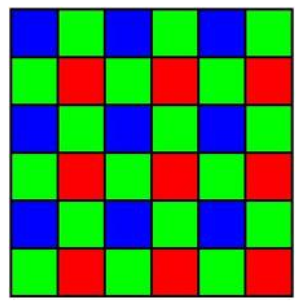
\includegraphics[scale=0.4]{./img/bayerarray.png}
		\par 
		\footnotesize\textit{Modelo de Bayer Array utilizado.}
	\end{center}
	\par 
	
Como podemos notar, e indexando las filas y columnas desde 0, los píxeles azules se encuentran en las posiciones de fila par y columna par. Por otro lado, el color rojo aparece en las filas impares y columnas impares, mientras que el color verde se encuentra en toda posición que no cumple la misma paridad entre columnas y filas.
\par 

\vspace{\baselineskip}

Una vez dicho esto, comenzamos con el análisis de las implementaciones realizadas para los siguientes filtros.
	
\subsubsection{Closest Neighbor}

Este filtro se basa en rellenar los valores faltantes copiando al vecino más
cercano del pixel, siempre y cuando tenga una observación real en el mismo canal que se está tratando averiguar. Este fundamento se basa en considerar que el valor de dos pixeles cercanos no debe variar mucho respecto de un mismo canal. De esta manera, podemos obtener toda la información que necesitamos a partir de contemplar el entorno de cada pixel.

\vspace{\baselineskip}

En nuestro caso, se decidió dividir los casos dependiendo si la información que buscamos corresponde al canal verde o a otro canal.

\vspace{\baselineskip}

Como ya se explicó previamente, el color verde va a ser encontrado en las columnas impares y filas pares al igual que en las columnas pares y filas impares. De esta manera, y mirando el modelo de bayer array que se planteó previamente, decidimos tomar los valores que se encuentra en la fila superior y misma columna, y los valores en la columna anterior y misma fila (es decir, tomar el valor del pixel justo encima y el que se encuentra justo a la izquierda). Sin embargo, a qué canal corresponde cada valor depende de en qué fila se encuentre el pixel que quiero reconstruir. Es por esto que se hace un chequeo sobre la fila del píxel.

\vspace{\baselineskip}

Solo a manera ilustrativa e informativa, se muestra en qué sector del código se realiza esto (método \textit{FilterImage()}): 

\vspace{\baselineskip}

\begin{lstlisting}
if (bayerImage.CurrentPixelIsGreen(i,j))
{
	greenChannelValue = bayerImage.GetPixel(i, j);
	blueChannelValue = getBlueChannelInGreenPixel(i, j);
	redChannelValue = getRedChannelInGreenPixel(i, j);
}
\end{lstlisting}

\vspace{\baselineskip}

Donde \textit{getBlueChannelInGreenPixel(i,j)} y \textit{getRedChannelInGreenPixel(i,j)} hacen la deferencia sobre en que fila se encuentra el pixel con valor de verde para devolver correspondientemente el color azul y rojo.

\vspace{\baselineskip}

Seguido, se plantea el caso en el que \textbf{NO} estamos ubicados en un pixel verde. Nuevamente, mirando el modelo utilizado para el bayer array, suceden dos casos: o el pixel es azul o es rojo. Sin embargo, en ambos se puede encontrar un pixel verde a su lado izquierdo (hay que ver cuestiones de bordes que serán explicadas a continuación). Y a su vez, en cualquier diagonal contigua podemos encontrar el otro color distinto de verde, es decir, al azul si estamos en rojo y viceversa. Elegimos tomar el valor que se encuentra en la diagonal superior izquierda. El código para esta parte es muy similar al mostrado previamente, solo que las condiciones son distintas. Igualmente, la asignación a las variables se hace de la misma forma.

\vspace{\baselineskip}

Podemos entonces distinguir en todo momento cuál es el color del pixel que estamos utilizando y qué posición vecina corresponde al mismo canal para tomar su valor. Cabe destacar que la elección de estos vecinos fue arbitraria. Dependiendo de la imagen que se utilice, algún vecino puede funcionar mejor que otra, pero esto no es cuantificable ni sigue un patrón tal que elegir un vecino en particular sea siempre la mejor opción.

\vspace{\baselineskip}

Dado que siempre estamos completando la información faltante a partir de los píxeles que se encuentran en la fila superior o la columna anterior (mirando de izquierda a derecha), el filtro comienza a aplicarse a partir de la segunda fila y la segunda columna. De esta manera, el primer caso será a partir de la posición $(1,1)$ de la matriz (indexada desde 0). Luego, en \textit{matlab} se le recorta el borde a la imagen, dejando sin utilización el borde para el cual se perdió la información.

\vspace{\baselineskip}

Finalmente, se setean los valores obtenidos a los canales correspondientes.



\subsubsection{Bilinear Interpolation}
Este método se compone de sucesivas interpolaciones lineales. De esta manera, se aproxima el valor de una función de dos variables a partir de puntos cercanos al que se quiere averiguar. En nuestro caso, esto se trasmite a cada pixel.  

\vspace{\baselineskip}

La interpolación lineal fue definida como \textit{$(aValue + anotherValue)/2$}, siendo $aValue$ y $anotherValue$ los valores de los pixeles que se desean interpolar. 

\vspace{\baselineskip}

Se define la interpolación bilineal como dos interpolaciones lineales, por ejemplo, una en las filas y otra en la columna, para luego interpolar linealmente ambos resultados. 

\vspace{\baselineskip}

Recordando que la estructura es Bayer Array, cuando nos encontramos con un pixel verde, podemos tener a ambos lados píxeles rojos o azules. Dependiendo de cual de estos casos cumplamos, arriba y abajo vamos a tener el color opuesto. De esta forma, cuando estemos en un pixel verde, se obtendrá el color azul interpolando linealmente vertical u horizontalmente (dependiendo de si estamos en fila par o impar), y en sentido opuesto para el rojo, obteniendo así los valores correspondientes a azul y rojo. Tengamos en cuenta que los colores rojos y azules se obtendrán en los métodos que se presentarán a continuación a través de esta interpolación.

\vspace{\baselineskip}

En el caso de estar en un pixel azul o rojo, tanto encima, abajo, a derecha e izquierda tenemos píxeles verdes. De esta manera, tomamos los cuatro píxeles verdes aledaños para realizar la interpolación; por un lado horizontal y por otro verticalmente, para luego finalizar interpolando ambos resultados. En estos casos, también debemos obtener el otro color distinto de verde, esto significa, obtener el azul para los píxeles rojos y viceversa. Para estos casos, desplazándose en cualquier diagonal podemos encontrar píxeles del color querido. Por lo que en nuestra implementación se hace una interpolación lineal para ambos pixeles en la fila anterior y otra para los de la siguiente fila. Finalmente, se interpolan entre ellos obteniendo el valor objetivo.

\vspace{\baselineskip}

La decisión de tomar los píxeles mencionados para realizar las interpolaciones, al igual que en \textit{Closest Neighbor}, fue arbitraria. El factor más influyente fue la cercanía entre píxeles, ya que, como se mencionó en la sección previa, se espera que los valores no varíen demasiado de un píxel a otro. De esta manera, interpolando los puntos cercanos se espera obtener un valor mucho más cercano que simplemente tomar alguno de los vecinos y utilizarlo.

\vspace{\baselineskip}

Debido a la forma en la que fue realizada el código, y gracias al polimorfismo, el código que resuelve el filtro de imagen es igual al utilizado en \textit{Closest Neighbor}, teniendo como única diferencia, que el valor de cada color obtenido es producto de interpolación tal como fue explicada previamente.

\subsubsection{Directional Interpolation}

Este método se basa en la interpolación por direcciones. En nuestro caso, esto implica interpolar valores obtenidos a partir de una dirección en la matriz. Respetando las consignas del TP, se decidió conseguir únicamente el canal verde a través de este método y para el resto de las canales se utiliza interpolación bilineal.

\vspace{\baselineskip}

En nuestro caso, utilizamos el gradiente para decidir si nos conviene tomar la dirección horizontal o vertical. Mientras mayor sea el gradiente, mayor es la variación de color entre un pixel y otro. El gradiente es útil por ejemplo, en los casos un pixel está junto a un borde: a priori, interpolar utilizando la información de una parte de la imagen que posiblemente no corresponda al mismo entorno del píxel en el cual trabajamos no parece una buena solución. Sin embargo, si tomamos la otra dirección, la cual posee menor gradiente, el resultado puede ser mejor. Decidimos entonces tomar los datos en la dirección de menor gradiente.

\vspace{\baselineskip}

El cálculo del gradiente se realiza utilizando la aproximación propuesta en el enunciado de este trabajo práctico. Básicamente, se consigue restando los valores del canal verde de los pixeles consecutivos (en la dirección vertical u horizontal) y tomando valor absoluto de ello.

\vspace{\baselineskip}

Como dijimos previamente, la información que queremos obtener es la correspondiente al canal verde de la imagen. De esta forma, cuando determinemos la dirección que deseamos, solo se interpolarán a partir de los píxeles verdes que conocemos. Se aplicará el algoritmo de interpolación a través de splines teniendo en cuenta como puntos únicamente a los píxeles verdes que ya poseemos su información en la fila o columna, dada por el criterio del gradiente.

\vspace{\baselineskip}

A través de splines (con el algoritmo obtenido del libro \textit{``Numerical Analysis'' de Richard L. Burden y J. Douglas Faires}) obtuvimos todos los polinomios correspondientes a la fila/columna respectiva al pixel del que deseamos obtener la información faltante. Con este algoritmo se consiguen todos los coeficientes de todos los trazadores cúbicos que interpolan cada par de puntos (polinomios cúbicos $S_j(x)$ en la teórica y la práctica). De esta forma obtenemos un polinomio que servirá para interpolar el canal verde en cualquier punto azul o rojo. En particular, podemos obtener el valor deseado para el pixel en el cual estamos iterando evaluando en el punto medio del polinomio interpolador correspondiente.

\subsubsection{Algoritmo de Malvar, He y Cutler}

El algoritmo de Malvar, He y Cutler se concentra en corregir la interpolación bilineal: para ello cada canal que se quiera conseguir va a ser calculado con el valor correspondiente a la interpolación bilineal, sumado a un factor de corrección basado en cálculos con el gradiente. Este factor se va a aplicar en una cierta medida $\alpha$ especificada como parámetro en este problema.

\vspace{\baselineskip}

Una vez más, nos concentraremos en obtener únicamente el canal verde con este método. El resto de los canales será calculado nuevamente a través de  interpolación bilineal.

\vspace{\baselineskip}

La corrección del gradiente se calcula esta vez en una vecindad más grande. Para conseguirla en este método aproximaremos el gradiente en una ventana de $5 \times 5$  y por lo tanto para empezar el algoritmo debemos asegurarnos que esta cantidad de vecinos siempre esté disponible. Para ello, tuvimos que eliminar 4 filas y 4 columnas (2 de cada lado), a diferencia de los otros filtros que permitían eliminar 2 filas y columnas.

\vspace{\baselineskip}

La fórmula exacta para esta corrección es la misma que la del paper de Malvar, He, Cutler [2]: 

\[ \hat{g}(i,j) = \hat{g}_B(i,j) + \alpha\Delta_R(i,j) \]

\vspace{\baselineskip}

A su vez como dijimos antes, esta corrección va a estar impuesta con cierta importancia gracias al parámetro $\alpha$. La fórmula resultante para el cálculo del valor del canal verde para un pixel en particular entonces es la siguiente:

\[ \Delta_R(i,j) \triangleq r(i,j) - \dfrac{1}{4} \sum_{\substack{
(m,n) = (0,-2) \\
(m,n) = (0,2) \\
(m,n) = (-2,0) \\
(m,n) =  (2,0)
  }} r(i+m, j+n) \]


\subsubsection{Problemas en la Implementación}
En este caso, no nos encontramos con problemas a la hora de realizar la implementación. Las decisiones de diseño tomadas, principalmente para que cada filtro se ejecute de la misma manera, fueron fundamentales a la hora de realizar el código. Permitió crear un programa legible, reducido, siendo sus problemas, fáciles de encontrar.

\vspace{\baselineskip}

Debemos notar que la utilización de \textit{MatLab} para preparar los datos para los algoritmos fue crucial para simplificar el problema.
	
\newpage
\subsection{Experimentación}

A la hora de decidir qué algoritmo se debe utilizar, hay varios puntos que se deben tener en cuenta. ¿Queremos que sea rápido? ¿Queremos una imagen que sea grata a la vista o preferimos que sea lo más semejante posible a la imagen que queremos capturar? ¿Es necesario ceder algo de tiempo a fin de obtener una mejor imagen? Y si es así, ¿Estamos dispuestos a hacerlo? 

\vspace{\baselineskip}

A continuación se plantearán estos problemas mostrando las diferencias cuantitativas y cualitativas de todos los algoritmos explicados previamente.

\subsubsection{Análisis Cuantitavo}

\begin{itemize}
\item \underline{PSNR:} 

La medición PSNR o \textit{Peak Signal to Noise Ratio} según sus siglas en inglés nos sirve para medir cuantitativamente la calidad de una imagen: este nos otorga un resultado en dB el cual indicará cuán buena es una imagen respecto de otra. Cuanto \textit{más grande} sea el resultado de aplicar PSNR para comparar imágenes, \textit{más parecidas} serán esas dos imágenes entre sí. Por lo tanto, al comparar dos imágenes idénticas, el resultado nos dará infinito. Se puede apreciar también en la fórmula de PSNR: 

\[ PSNR(I_1, I_2) = 20 \cdot log_{10}(255) - 10 \cdot log_{10}(MSE(I_1, I_2)) \]

Donde $MSE$ es el error cuadrático medio (\textit{Mean Squared Error}, en inglés) y se calcula de la siguiente manera:

\[ MSE(I_1, I_2) = \dfrac{1}{mn} \sum\limits_{i=0}^{m-1}\sum\limits_{j=0}^{n-1}[I_1(i,j) - I_2(i,j)]^2 \]

De aquí se puede apreciar que si las imágenes son idénticas, el error cuadrático medio se hace 0 y hacer el logaritmo de 0 no es válido, por lo tanto PSNR devuelve en ese caso infinito.


Luego para nuestro problema, comparamos las imágenes filtradas con cada filtro contra las 12 imágenes provistas por la cátedra. Además, separamos el análisis para la capa verde únicamente como para todas las capas. Ambas opciones estarán involucradas en este análisis.

Fue entonces realizado el score de PSNR para todos los filtros, para la capa verde y todas las capas, y para todas las imágenes provistas. Para tener una observación general se tomó la media de todos los resultados según el filtro. Este es el gráfico resultante:

	\begin{center}
		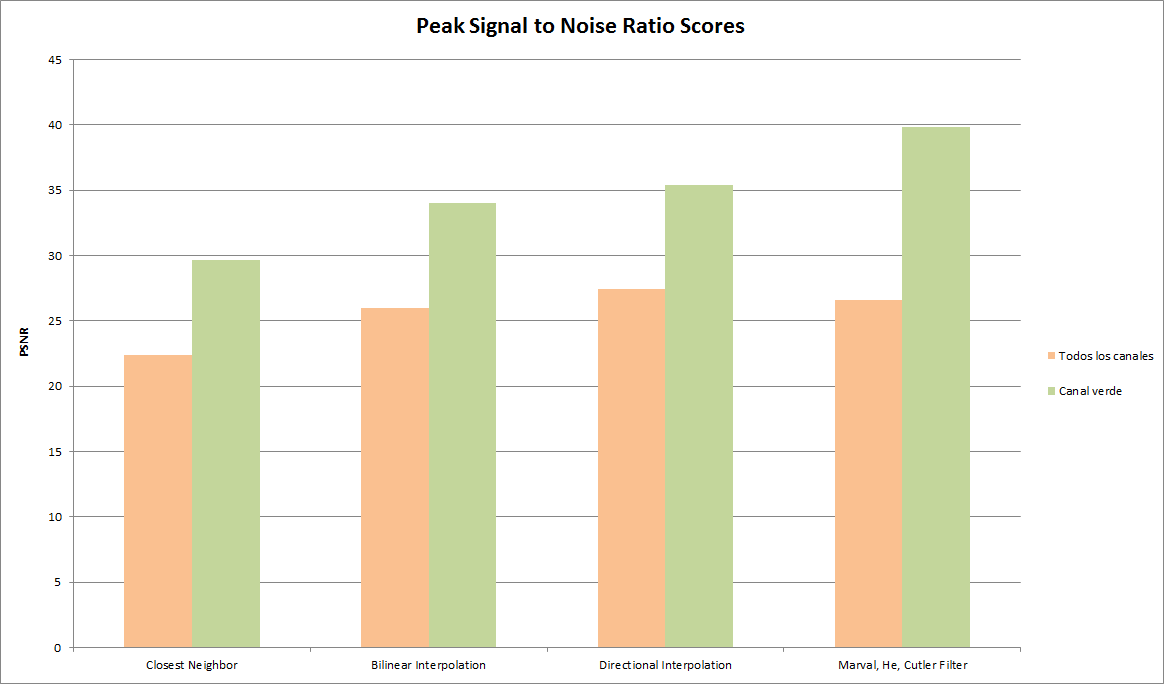
\includegraphics[scale=0.27]{./img/psnrScores.png}
		\vspace{2pt}
		\par
		\footnotesize\textit{Media de todos los resultados de PSNR aplicado a todas las imágenes provistas para todos los filtros}
	\end{center}


Antes que nada hay que aclarar que la diferencia de score entre todos los canales y el canal verde existe y da mejor para el canal verde es porque, tal como se nos explicó en la presentación del TP, los humanos percibimos mejor este color y por lo tanto el bayer array tiene más verde que los otros colores. Además, al concentrarnos primordialmente en este canal para la gran mayoría de los filtros, es normal que el resultado tenga esta forma.

Podemos ver entonces que para esta medida de calidad, el algoritmo más \textit{naïf} es el de peor rendimiento, llegando aproximadamente a los 29 dB. Luego, la interpolación bilateral nos consigue un valor de 34 dB. La interpolación direccional con splines empata en esta medición. Finalmente, el algoritmo de Malvar, He y Cutler, el cual aplica una corrección basada en el gradiente al filtro bilineal, es el que mejor funcionó, llegando a rozar el pico de los 40 dB. De aquí nos llevamos que claramente para PSNR el algoritmo de Malvar, He y Cutler es el ganador, mientras que interpolar direccionalmente (horizontalmente y verticalmente) toda una fila y una columna con splines contra interpolación bilineal en una vecindad de $3 \times 3$  nos da prácticamente los mismos resultados (34,00147845 para bilineal y 34,01162873 para direccional, una diferencia \textit{extremadamente chica}). Por lo tanto, si debemos elegir entre estos dos algoritmos, esta elección dependerá del tiempo de cómputo y de los \textit{artifacts} visuales que aparezcan (sin tener en cuenta la otra medición SSIM). Adelantándonos al análisis de tiempo de cómputo de los algoritmos, podemos intuir rápidamente que el filtro bilineal será mucho rápido que splines, ya que este último implica resolver matrices versus operaciones sencillas de interpolación lineal.

Si miramos ahora los valores de todos los canales, se puede notar, además de tener valores más bajos, que el orden de la performance de los algoritmos según PSNR es el mismo. Debemos recordar también que conseguir los colores rojo y azul con las interpolaciones de Malvar, He y Cutler y \textit{Directional Interpolation} se realizó en ambos casos de igual manera con interpolación bilineal. Esto tal vez explique también el parecido en los scores entre interpolación direccional e interpolación bilineal. Para Malvar, He y Cutler, esto seguramente signifique que la mejora para todos los canales fue mejorada gracias a la mejora del verde y nada más.

\vspace{\baselineskip}

Sin embargo, este análisis está basado en \textbf{la media de todos los resultados para todas las imágenes.} En este caso, si nos ponemos a mirar la tabla completa con todos los valores, veremos que este orden se mantiene \textit{para cada una de las imágenes}. Las interpolaciones bilineales y direccionales son las únicas que no tienen bien definido cuál es mejor en términos de PSNR, ya que hay imágenes en las que funciona mejor bilineal que direccional y vice versa. De cualquier forma, analizar estos casos no tiene mucho sentido (para PSNR) ya que la diferencia es mínima. Todos estos valores, incluídos las medias y los gráficos están en un archivo de \textit{Excel} en la carpeta \textit{informe/excel/}.

\vspace{\baselineskip}

De aquí nos llevamos entonces que, siguiendo únicamente los scores de PSNR, \textit{Closest Neighbor} definitivamente no es el algoritmo que querríamos usar para obtener una imagen de buena calidad. Entre interpolación bilineal y direccional no hay mucha diferencia (habiendo interpolado en esas direcciones y esa cantidad de puntos que discutimos en la sección de implementación), pero ambos son mejores que \textit{Closest Neighbor}. El algoritmo a elegir es entonces el de Malvar, He y Cutler, el cual tiene el mejor PSNR. Faltará decidir nada más si este algoritmo conviene a nivel de tiempos de cómputo, análisis que será desarrollado posteriormente.

\item \underline{SSIM:}

SSIM o \textit{Structural Similarity} es otro tipo de medición de calidad entre dos imágenes. Este medidor se jacta en concentrarse más en lo visualmente parecido que en lo parecido matemáticamente/matricialmente, siendo esta última una crítica al PSNR y al error cuadrático medio. Ambos PSNR como SSIM tienen en común que, cuanto más alto sea el valor devuelto, más se parecen las imágenes comparadas. Esta vez, el valor máximo para SSIM es 1, luego las imágenes cuyo valor al aplicar este medidor sea más cercano a 1 serán las más parecidas a la imagen original en los criterios de SSIM. Se pueden ver más detalles de SSIM y la implementación que usamos\footnote{En particular los valores fueron calculados de la forma \textit{ssim(img1, img2)} sin parámetros adicionales.} en la referencia [4]. 

El análisis se realizó de la misma manera que para PSNR: es decir, tomamos los resultados de aplicarlo a todas las imágenes con todos los filtros para el canal verde y para todos los canales. Para ver un resultado general, de manera análoga, tomamos la media de los resultados. He aquí el gráfico correspondiente:

	\begin{center}
		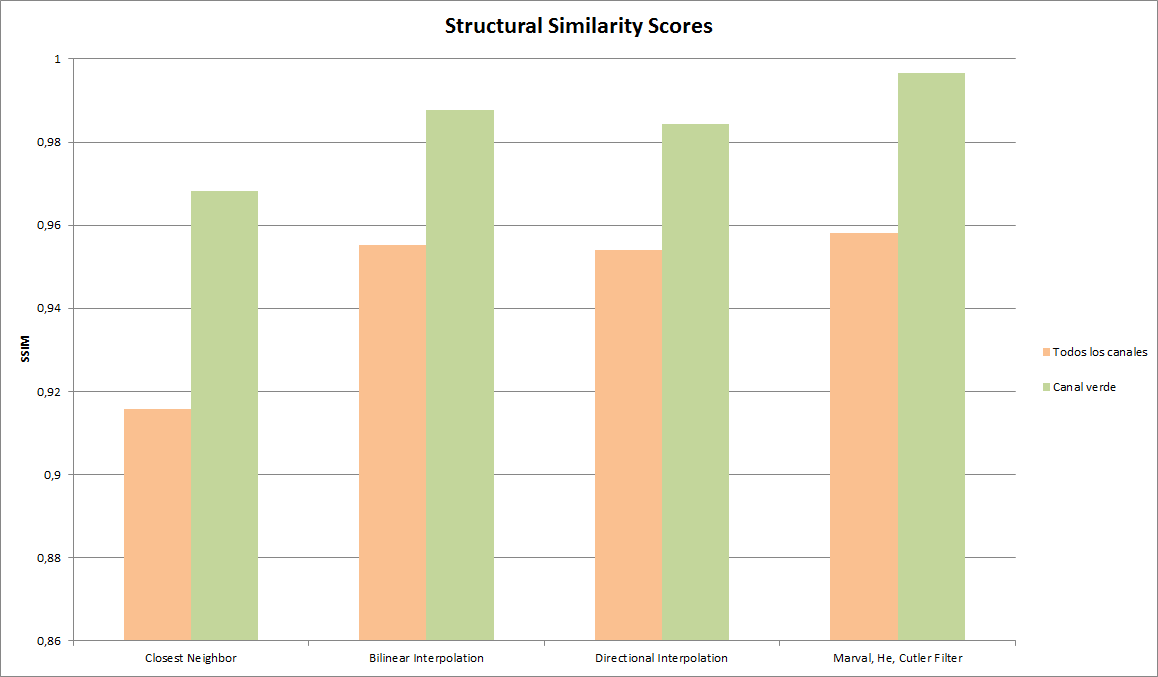
\includegraphics[scale=0.3]{./img/ssimScores.png}
		\vspace{2pt}
		\par
		\footnotesize\textit{Media de todos los resultados de SSIM aplicado a todas las imágenes provistas para todos los filtros}
	\end{center}
	
Ya que el gráfico se mira de la misma manera que el de PSNR (cuanto más mejor), podemos observar rápidamente que los resultados \textit{se repiten}. Un dato más que se puede apreciar es que sin importar quién lidere en este gráfico, todos los valores son muy cercanos a 1, por lo tanto podemos esperar que las imágenes filtradas sean \textit{visualmente} parecidas a la original en un vistazo rápido. 

Nos queda entonces que el claro perdedor resulta ser \textit{Closest Neighbor} y el ganador definitivo Malvar, He y Cutler. Sin embargo, esta vez es \textit{Bilineal Interpolation} el que sale en segundo lugar, dejando atrás \textit{Directional Interpolation} con SPLINES sobre filas y columnas. Aparentemente para SSIM, las imágenes con este último algoritmo de \textit{demosaicing} son menos parecidas a la original que utilizando \textit{Bilinear Interpolation}. Sabiendo además que SSIM supuestamente tiene mejor en cuenta cuán parecida es una imagen para el ojo humano, podríamos decir que aquellas pasadas por \textit{Directional Interpolation} son menos parecidas estructuralmente a la vista.


\item \underline{Análisis de tiempos:}

Ya vimos qué algoritmos brindan una imagen con mayor similitud a la original. Ahora nos tenemos que plantear qué tiempos de cómputo corresponden a cada uno de los métodos realizados. 

La experimentación realizada para calcular los tiempos de cada método se realizó teniendo en cuenta sólo el tiempo de cómputo del color verde. Esto se debe a que tanto la interpolación direccional como el algoritmo de Malvar, He y Cutler obtienen la información faltante de los colores rojo y azul a través del algoritmo de interpolación bilineal. De esta forma, pierde sentido analizar su tiempo de cómputo ya que es simil para todos.

Lo primero que notamos al realizar esta experimentación fue que se obtuvieron mediciones muy similares para el mismo algoritmo aplicado a las distintas imágenes presentadas por la cátedra. Esto se puede ver reflejado en los siguientes gráficos:

	\begin{center}
		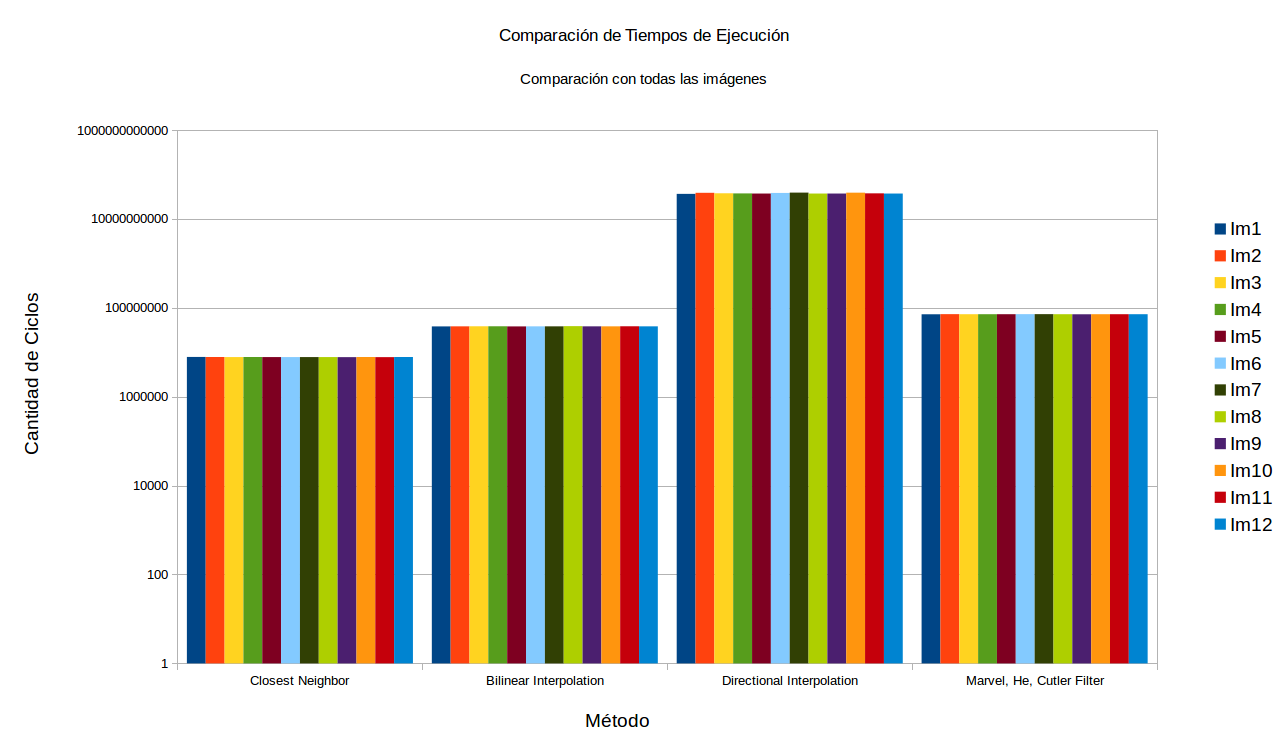
\includegraphics[scale=0.4]{./img/comparacionMetodoImagen.png}
		\vspace{2pt}
		\par
		\footnotesize\textit{Comparación entre imágenes y algoritmos para un promedio de 20 repeticiones del método.}
	\end{center}

Como podemos notar, para un mismo algoritmo, \textbf{TODAS} las imágenes brindadas por la cátedra obtienen un promedio de 20 iteraciones del algoritmo muy similar. Esto implica que el tiempo de cómputo \textbf{NO} depende de la imagen, sino que solamente del algoritmo utilizado, claro está, a igual dimensión. 

Teniendo en cuenta las implementaciones de los filtros, es coherente siendo que no se deben realizar distinta cantidad de instrucciones dependiendo de características de la imagen. El único caso en el que puede verse alguna particularidad como esta sería con el algoritmo de interpolación direccional. Recordemos que a partir del valor del gradiente obtenido en dirección horizontal y vertical al pixel, se toma una fila o una columna respectivamente. A partir de esta elección se toma todo el vector fila o columna y se realiza splines sobre eso. De todas formas, las imágenes poseen similar altura y ancho.

Supongamos imágenes mucho más anchas que altas; por ende, la matriz que representa la imagen va a ser rectangular. Además, diferenciemos dos imágenes tal que el algoritmo de interpolación siempre posea el menor gradiente en la dirección columna mientras que la otra imagen la posea siempre en las filas. En este caso, la diferencia de tiempo será la causada por el cálculo de splines. Teniendo en cuenta que la complejidad de este algoritmo es O($n + log(n)$)[3], la potencial diferencia entre la cantidad de columnas y filas se verá influenciada en un orden lineal (siendo el $n$ lo que predomina en esta complejidad).

Sin embargo, no existen imágenes infinitas, y solamente el cálculo de splines es el que puede modificar de alguna manera el tiempo de cómputo. Pero para imágenes ``normales'', donde no se produce ningún caso extraño y el cálculo del gradiente alterna la elección del vector sobre el que aplicar splines, los tiempos de cómputo, como se vieron en la experimentación realizada.


\vspace{\baselineskip}

Estamos analizando el promedio de iteraciones para cada imagen dependiendo del algoritmo. Los valores son muy similares para el mismo algoritmo. De esta manera, si calculamos la cantidad de ciclos promedio del algoritmo, nos encontraremos con un gráfico muy similar al recién mostrado:

	\begin{center}
		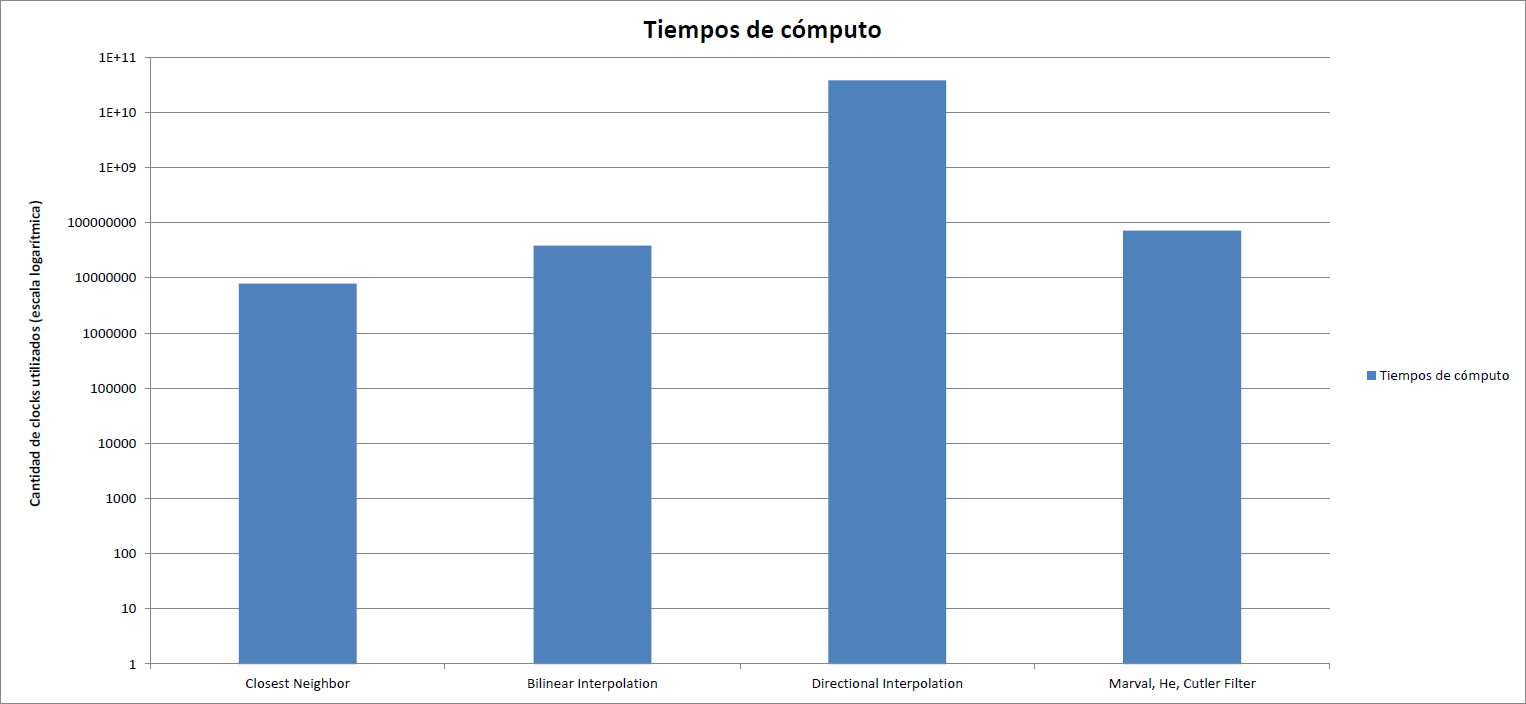
\includegraphics[scale=0.4]{./img/tiemposDeComputo.png}
		\vspace{2pt}
		\par
		\footnotesize\textit{Comparación de cantidad de ciclos promedio para cada método.}
	\end{center}

Este gráfico se corresponde con el obtenido a partir de los promedios de cada imagen. Ya que interpretamos que una corrida del algoritmo casi no varía de una imagen a otra, y tenemos 20 corridas por algoritmo por cada una de las 12 imágenes, consideramos cantidad suficiente para calcular un promedio por algoritmo.

\vspace{\baselineskip}

Como se puede ver, la cantidad de ciclos utilizada por \textit{Closest Neighbor} es la menor a todas. De esta manera vemos que, lo que perdimos en cuenta a la similitud con la imagen original lo estamos ganando en velocidad. Es por esto que puede plantearse una situación donde este sea el método que mejor se acomoda a las circunstancias. 

\vspace{\baselineskip}

Por otro lado, vemos una relación muy parecida entre el método de \textit{interpolación bilineal} con el \textit{algoritmo de Malvar, He y Cutler}. Esto es razonable debido a que este último método se basa en aplicar una interpolación bilineal a la cual le realiza operaciones para modificar su calidad. Así vemos que con un leve aumento del tiempo de cómputo, podemos obtener una imagen de mayor calidad. A pesar de esto, el método de interpolación bilineal resulta más costoso que el de Closest Neighbor pero teniendo en cuenta la calidad de la imagen, puede preferirse ceder algo de tiempo para obtener una mayor nitidez o menor cantidad de artifacts. Teniendo en cuenta que la diferencia de tiempos de cómputo entre ambos no es tan notoria, y que también la implementación del algoritmo de Closest Neighbor se basa en el azar de obtener un buen vecino, la interpolación bilineal se vuelve un buen candidato a utilizar.

\vspace{\baselineskip}

Por último, tenemos la \textit{interpolación direccional}. Esta última obtiene muy buenos resultados de calidad, sin embargo el tiempo de cómputo es muy alto y extensamente alejado de los demás métodos presentados.
Sin embargo, puede ser una buena elección si tenemos el tiempo para procesarlo. El usuario podría obtener una imagen de mayor calidad y más gustosa a la vista. 

\vspace{\baselineskip}

Este último planteo nos deja a la vista más preguntas. Tenemos un análisis que nos dice que métodos nos brindan imágenes más cercanas a la original. Podemos a su vez decidir si queremos gastar el tiempo para obtener una imagen más ``real'' o no. Sin embargo, ¿es eso lo que queremos? ¿Qué es lo que se busca: una imagen más real o una imagen que se vea bien? Ya vimos que para obtener una o la otra es necesaria gastar más o menos tiempo en cómputo, pero ahora nos planteamos algo que se aleja de lo cuantificable. 

\vspace{\baselineskip}

Por lo tanto, pasamos a preguntarnos: ¿me gusta la imagen o no?

\end{itemize}

\newpage

\subsubsection{Análisis Cualitativo}

Para la búsqueda de \textit{artifacts} corrimos los cuatro algoritmos sobre las imágenes de la cátedra y proseguimos a buscarlos de manera empírica. Encontramos casos donde cada algoritmo funciona mejor que el resto, donde ``mejor'' queda sujeto a nuestra interpretación, subjetiva.

\vspace{\baselineskip}

La primer imagen utilizada es la de los loros \textit{(img1.bmp)}: nos quedamos sólo con el borde entre el fondo verde y el pico del loro que se encuentra a la derecha. Vemos como trata cada algoritmo la diferencia de tonalidad al presentarse una recta. 

\vspace{\baselineskip}

	\begin{center}
		
\includegraphics[scale=.5]{../enunciado/images_files/cualitativo/pico_loro_closest.png}
		\vspace{2pt}
		\par
		\footnotesize\textit{Borde entre colores, algoritmo: Closest Neighbor.}
	\end{center}

	\begin{center}
		
\includegraphics[scale=.5]{../enunciado/images_files/cualitativo/pico_loro_bilinear.png}
		\vspace{2pt}
		\par
		\footnotesize\textit{Borde entre colores, algoritmo: Bilinear Interpolation.}
	\end{center}

	\begin{center}
		
\includegraphics[scale=.5]{../enunciado/images_files/cualitativo/pico_loro_directional.png}
		\vspace{2pt}
		\par
		\footnotesize\textit{Borde entre colores, algoritmo: Directional Interpolation.}
	\end{center}


	\begin{center}
		
\includegraphics[scale=.5]{../enunciado/images_files/cualitativo/pico_loro_malvar.png}
		\vspace{2pt}
		\par
		\footnotesize\textit{Borde entre colores, algoritmo: Malvar He Cutler.}
	\end{center}

\vspace{\baselineskip}

 \textit{Closest Neighbor}  posee notoriamente el artifact conocido como ``zipping''. Esto se debe intrínsecamente a cómo se obtienen los píxeles para rellenar; al copiar el valor de un píxel lindero, cuando nos encontramos en un borde, este, no va ser homogéneo. En el lado más claro se agrupan píxeles dando la sensación de tener conjunto de ``ladrillos'' del mismo color, su justificación es la misma que la del borde, simplemente con distintos tonos del mismo color.

En el algoritmo \textit{Bilinear} la imagen es mucho mas homogénea ya que se utiliza la interpolación de cuatro puntos, ponderando así el valor de un píxel mediante la utilización de varios vecinos.

\textit{Directional interpolation} devuelve la imagen más suave. Recordemos que interpola por \textit{splines} en la dirección con deriva más chica, en este caso la vertical. 

El último algoritmo \textit{Malvar, He, Cutler}, posee las misma propiedades que el bilinear pero siendo más suave.

\vspace{\baselineskip}

A continuación veremos un extracto la la imagen número once (suministrada por la cátedra), correspondiente a la pared de un granero.

\vspace{\baselineskip}

%.---------------------
	\begin{center}
		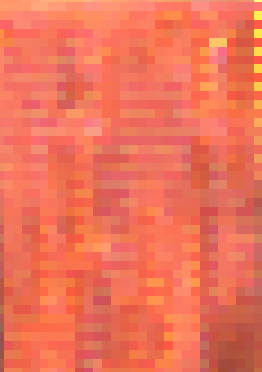
\includegraphics[scale=.5]{../enunciado/images_files/cualitativo/farm_closest.png}
		\vspace{2pt}
		\par
		\footnotesize\textit{Pared de un granero iluminado por el atardecer, algoritmo: Closest Neighbor.}
	\end{center}


	\begin{center}
		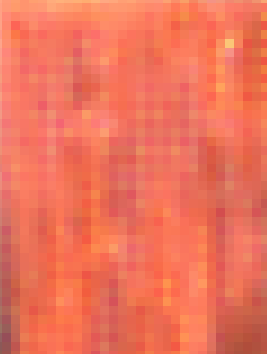
\includegraphics[scale=.5]{../enunciado/images_files/cualitativo/farm_bilinear.png}
		\vspace{2pt}
		\par
		\footnotesize\textit{Pared de un granero iluminado por el atardecer, algoritmo: Bilinear Interpolation.}
	\end{center}


	\begin{center}
		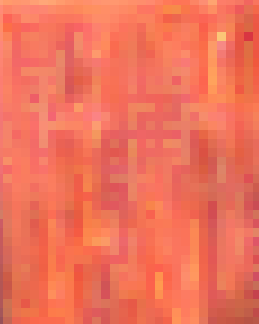
\includegraphics[scale=.5]{../enunciado/images_files/cualitativo/farm_directional.png}
		\vspace{2pt}
		\par
		\footnotesize\textit{Pared de un granero iluminado por el atardecer, algoritmo: Directional Interpolation.}
	\end{center}


	\begin{center}
		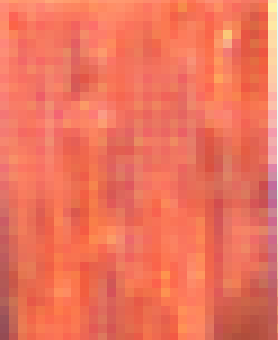
\includegraphics[scale=.5]{../enunciado/images_files/cualitativo/farm_malvar.png}
		\vspace{2pt}
		\par
		\footnotesize\textit{Pared de un granero iluminado por el atardecer, algoritmo: Malvar He Cutler.}
	\end{center}

\vspace{\baselineskip}

El algoritmo de vecinos mas cercanos y el de interpolación direccional poseen los \textit{artifacts} más notorios. En el primero volvemos a ver la creación de bloques similares a ladrillos en una pared y en el segundo la aparición de laberintos en la imágen.

Consideramos que el algoritmo bilinear devuelve una mejor solución que \textit{Malvar He Cutler} considerando cómo manejan la anomalía de la esquina superior derecha (punto blanco). Dado que el segundo utiliza una vecindad extendida para definir el valor de cada píxel, si se encuentran detalles en la imagen que son resonantes (como un punto de otro color) el algoritmo los propaga de manera más notoria que el bilineal.

\vspace{\baselineskip}

Encontramos una imagen donde los artifacts que generan los algoritmos más complejos son más notorios y nos llevan a elegir como imagen de mejor calidad a la que le fue aplicada vecinos más cercanos. El extracto de imagen corresponde a rejas blancas, siendo la imagen número ocho suministrada por la cátedra.

%.---------------------

	\begin{center}
		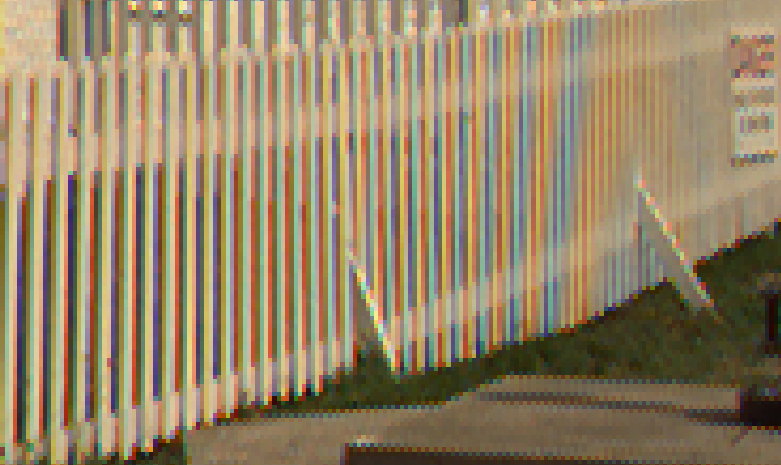
\includegraphics[scale=.5]{../enunciado/images_files/cualitativo/pharo_rails_closest.png}
		\vspace{2pt}
		\par
		\footnotesize\textit{Rejas blancas, algoritmo: Closest Neighbor.}
	\end{center}


	\begin{center}
		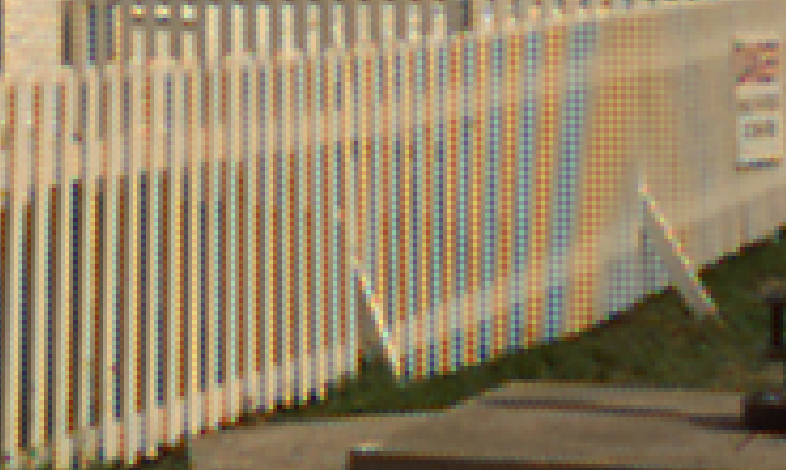
\includegraphics[scale=.5]{../enunciado/images_files/cualitativo/pharo_rails_bilinear.png}
		\vspace{2pt}
		\par
		\footnotesize\textit{Rejas blancas, algoritmo: Bilinear Interpolation.}
	\end{center}


	\begin{center}
		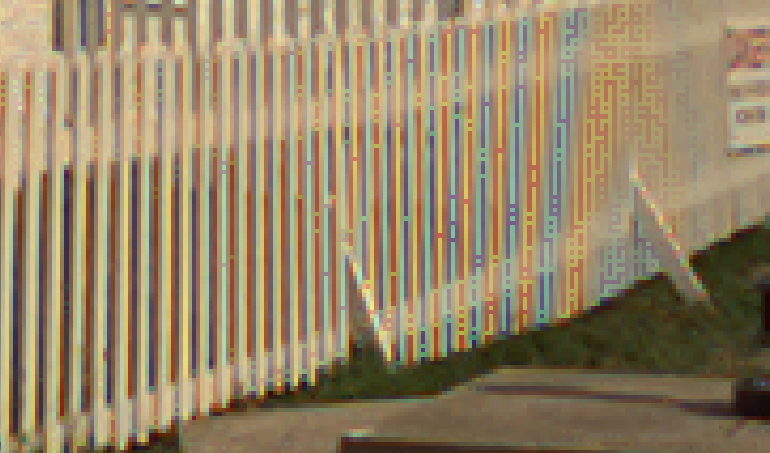
\includegraphics[scale=.5]{../enunciado/images_files/cualitativo/pharo_rails_directional.png}
		\vspace{2pt}
		\par
		\footnotesize\textit{Rejas blancas, algoritmo: Directional Interpolation.}
	\end{center}


	\begin{center}
		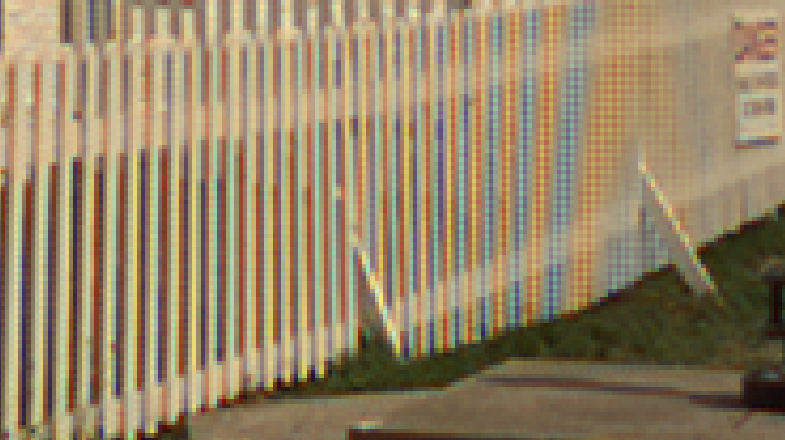
\includegraphics[scale=.5]{../enunciado/images_files/cualitativo/pharo_rails_malvar.png}
		\vspace{2pt}
		\par
		\footnotesize\textit{Rejas blancas, algoritmo: Malvar He Cutler.}
	\end{center}

\vspace{\baselineskip}
El algoritmo bilineal y de Malvar poseen los mismo artifacts, generando la cuadrilla. El direccional genera el laberinto, los tres mencionados previamente. Lo interesante es lo que le pasa al algoritmo de vecinos más cercanos: Dada la rectitud de las rejas, y como se copia el color de al lado, el patrón se mantiene en la misma dirección que las rejas. Mirando esta imagen pero en resolución original (sin \textit{zoom}), este algoritmo nos da el resultado más agradable a la vista.


\vspace{\baselineskip}

%.--------------------
Encontramos en la imagen de las palmeras (número siete) un artifact llamativo para el algoritmo direccional, y sólo se incluye ella, dado que los otros algoritmos no aportan información nueva.

	\begin{center}
		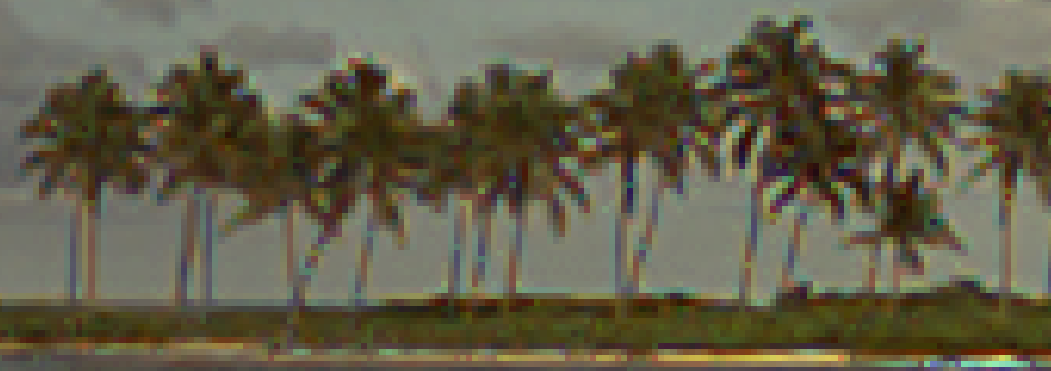
\includegraphics[scale=.5]{../enunciado/images_files/cualitativo/palms_directional.png}
		\vspace{2pt}
		\par
		\footnotesize\textit{Palmeras en el horizonte, algoritmo: Directional Interpolation.}
	\end{center}

\vspace{\baselineskip}

Pareciera que algunos píxeles correspondientes a los troncos de las palmeras fueron tapados con el fondo, y por eso las palmeras ``flotan''. Parece ser un nuevo artifact ya que hasta el momento sólo habíamos encontrado el laberinto para el direccional. Dado que con esta información no podemos asegurar nada en concreto, procedemos a efectuar un \textit{zoom} sobre uno de los troncos.

\vspace{\baselineskip}

	\begin{center}
		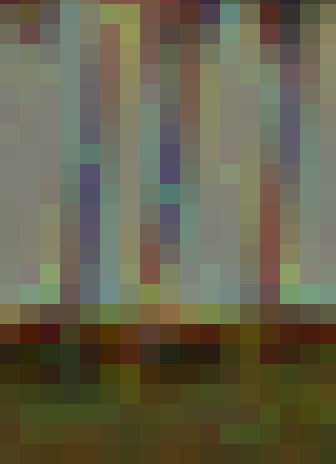
\includegraphics[scale=.5]{../enunciado/images_files/cualitativo/palms_zoom_directional.png}
		\vspace{2pt}
		\par
		\footnotesize\textit{Zoom sobre uno de los troncos para imagen de palmeras, algoritmo: Directional Interpolation.}
	\end{center}

\vspace{\baselineskip}

Podemos ver que tanto el pasto (verde en la parte inferior) y el fondo azul forman laberintos. Así mismo, el correspondiente al fondo realiza su recorrido pasando por el tronco y de esta manera generando la ilusión de que estan cortados. Concluímos entonces que no encontramos un nuevo artefacto.

\vspace{\baselineskip}

Hemos encontrado distintos casos donde cada algoritmo nos da un mejor resultado que el otro. En lineas generales, vecinos cercanos no es un bueno, salvo el caso de las rejas: posee zipping muy notorio. En cambios abruptos de color en lineas rectas, el algoritmo de interpolación direccional da los mejores resultados. Por otro lado, Malvar y bilineal dan similares resultados, siendo el primero una mejora del segundo. Mirando las imágenes completas y sin zoom, Malvar y direccional parecen dar las imágenes con mejor calidad. Sólo cuando se pasa al detalle que Malvar supera a direccional ya que el artefacto del laberito aparece.

Se encontraron artifacts en varias de las imágenes proveídas por la cátedra que no se agregaron al informe al no aportar más información. Las mismas están dentro de la carpeta \texttt{cualitativo}.


\newpage

\section{Conclusión}

Lo interesante a destacar es, que hilando fino, podemos ver que ninguna de las imágenes son iguales. La digitalización de las imágenes nos otorga una mirada sesgada e irreal de la realidad (considerando ``realidad'' como lo que nuestros ojos pueden interpretar).

[COMPLETAR]
\par
[COMPLETAR]
\par
[COMPLETAR]
\par
[COMPLETAR]

\newpage

\section{Bibliografía y referencias} 

\begin{itemize}
	\item \textbf{STL de C++}: \url{http://en.cppreference.com}.
%	\par Para la función \texttt{rand()}, \url{http://en.cppreference.com/w/cpp/numeric/random/rand}.
%	\par Para la función \texttt{sort()}, \url{http://en.cppreference.com/w/cpp/algorithm/sort}.
%	\item Distribución de \texttt{rand()}?, \url{http://eternallyconfuzzled.com/arts/jsw\_art\_r and.aspx}
%	\item \textbf{Métodos Numéricos:}
%		\par Método de la potencia: Richard BURDEN, Numerical Analysis 9th Ed. Chapter 9 Section 3, p. 576
%		\par \textit{Papers} del TP.
%	\item \textbf{Contador de clocks}: \url{http://www.mcs.anl.gov/\~kazutomo/rdtsc.html}
\item \ [1] \ Cambridge in Colour:  \url{http://www.cambridgeincolour.com/tutorials/camera-sensors.htm}
\item \textbf{Métodos Numéricos:}
		\par [2] Resolviendo SPLINES eficientemente: Richard BURDEN, Numerical Analysis 9th Ed. Chapter 3, p. 150
\item \ [3] Más información sobre la complejidad de las interpolaciones: \ \url{http://www.csie.ntu.edu.tw/~lyuu/theses/thesis\_r91723055.pdf}
\item \ [4] \ SSIM:  \url{https://ece.uwaterloo.ca/\~{}z70wang/research/ssim/}

\item \ [5] Más sobre medidas de calidad (PSNR, SSIM y más): \url{http://www.ijser.org/researchpaper\%5CComparison-of-Image-Quality-Assessment-PSNR-HVS-SSIM-UIQI.pdf}

\end{itemize}


\end{document}
